\bookchapter{第六十章：築開發之環境——Xcode 與第一個項目}

\chapterintro{工欲善其事，必先利其器。此章吾儕先築「庖廚」：裝成 Xcode、跑通模擬器、創人生第一個 iOS 項目，再拆工程之結構而觀之明白。環境既成，爾將初見己所書之代碼化為可點之鈕——此一瞬，多人記之終身。}

\booksection{一、備 Mac 一台}

先言其檻：iOS 開發必於 macOS 之上行之。爾若無 Mac，其擇有三：購一台（縱二手之 Mac mini 或 MacBook Air 亦足用）、短期租雲上之 Mac、或先讀第八篇《安卓開發實戰篇》（Windows 即可為之）。

\begin{center}
\begin{tabularx}{\linewidth}{|X|X|X|}
\hline
\textbf{配置之項} & \textbf{至低之要求} & \textbf{寬裕之線（所薦）} \tabularnewline
\hline
晶片 & Apple Silicon（M1 起） & M2 及更新 \tabularnewline
記憶體 & 8GB & 16GB \tabularnewline
磁碟 & 預留 40GB 以上（Xcode 本體甚巨） & 256GB 起步 \tabularnewline
系統 & 最新之 macOS & 常保自動更新 \tabularnewline
\hline
\end{tabularx}
\end{center}

\begin{center}\small\color{gray}Mac 開發機配置參考（2026 年 8 月）\end{center}

\begin{tcbinfo}{小訣：無 Mac 亦能先學語言}
iPad 之上免費之 Swift Playgrounds 可學 Swift 語言之基（不必 Mac）；即 iPhone 之上亦可裝之。先於 Playgrounds 之中玩熟第 61 章語言之知識，待得 Mac 則徑起飛矣。磨刀不誤砍柴之工，此之謂也。

\end{tcbinfo}

\booksection{二、安裝 Xcode}

Xcode 者，蘋果官方集成開發之環境也，免費。三步裝成：

\begin{enumerate}
  \item 於 Mac 開 App Store，搜「Xcode」，點而安裝之——注意其有好幾 GB 之巨，擇網速善之時段；
  \item 裝畢首次啟動，允其協議、裝畢組件（自動而成）；
  \item 菜單 Xcode Settings Locations，確認 Command Line Tools 已選——命令行之器，乃多腳本與第三方之器之前提也。
\end{enumerate}

\begin{tcbwarn}{注意：版本與系統之「匹配遊戲」}
新 Xcode 往往須最新之 macOS，舊 Mac 則滯於舊版。上架 App Store 之時，蘋果必求以較新之 Xcode 構建（通常予一寬限之期）。故系統之更新勿拖太久——iOS 開發者乃「追新版」至勤之一群也。

\end{tcbwarn}

\booksection{三、創爾之第一個項目}

開 Xcode Create New Project 擇 iOS App 之範本，而後填之：

\begin{center}
\begin{tabularx}{\linewidth}{|X|X|X|}
\hline
\textbf{配置之項} & \textbf{填何物} & \textbf{說明} \tabularnewline
\hline
Product Name & MyFirstApp & 應用之名 \tabularnewline
Team & 爾之 Apple ID（免費） & 簽名所用，個人帳號即可 \tabularnewline
Organization Identifier & com.example & 與 Product Name 併為包之標識 \tabularnewline
Interface & SwiftUI & 本書主線之框架 \tabularnewline
Language & Swift & 毋庸贅釋 \tabularnewline
\hline
\end{tabularx}
\end{center}

\begin{center}\small\color{gray}創建項目所填之五事\end{center}

點 Create 之後，Xcode 將生一可徑行之項目。左上角擇模擬器一台（如 iPhone 17），點 > 而運行——數秒之後，模擬器之屏現一書「Hello, world!」之窗。爾之第一個 iOS App 誕生矣。

\booksection{四、拆工程之結構：每文件何為}

左側乃工程導航之器，新手但識此數者可也：

\begin{center}
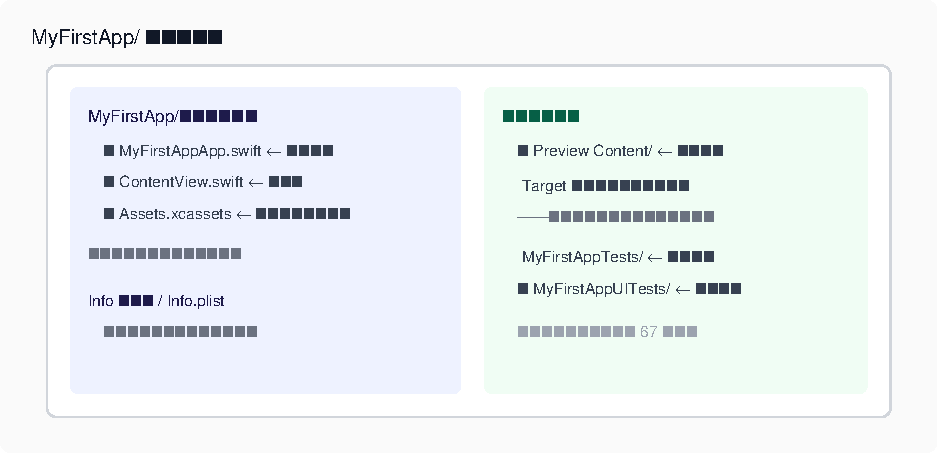
\includegraphics[width=0.92\linewidth]{figures/fig-di-liu-shi-zhang-1}
\\[2pt]\small 圖二：新手必懂之 Xcode 工程結構
\end{center}

\begin{itemize}
  \item MyFirstAppApp.swift：程序之入口，SwiftUI 之中惟數行——「啟之，而後示主界面」；
  \item ContentView.swift：主界面之視圖，爾今所見皆在此；
  \item Assets.xcassets：資源之倉——圖標、圖、色皆置於此；
  \item Target 之設置：點左側藍色工程之圖標而入，版本之號、至低 iOS 之版本、簽名皆在其中。App 顯示之名、圖標亦於此配置。
\end{itemize}

\booksection{五、真機調試：裝 App 於爾之 iPhone}

\booksection{五、Xcode 效率之技：新手之五「快捷鍵外掛」}

熟用此數者，爾將顯得「甚專業」：

\begin{center}
\begin{tabularx}{\linewidth}{|X|X|X|}
\hline
\textbf{操作} & \textbf{快捷鍵} & \textbf{功用} \tabularnewline
\hline
運行 & CmdR & 編譯並跑之 \tabularnewline
開/切畫布之預覽 & OptionCmd & 所見即所得之開關 \tabularnewline
格式化縮進 & CtrlI & 自整所選代碼之縮進 \tabularnewline
快速開文件 & CmdO & 輸入文件之名而秒開（至常用！） \tabularnewline
註釋/取消註釋 & Cmd/ & 調試之時隨手開關代碼 \tabularnewline
\hline
\end{tabularx}
\end{center}

\begin{center}\small\color{gray}Xcode 高頻快捷鍵（新手五件套）\end{center}

又有兩個隱藏之福利：多開模擬器（同時跑 iPhone 與 iPad 以比其佈局）與代碼片段之庫（以常用之數行拖入右側 Snippets 之面板，下次一鍵插入）——效率之器先用之，手感自來矣。

\booksection{六、真機調試：裝 App 於爾之 iPhone}

模擬器雖善，真機方為終點。以免費之 Apple ID 亦可真機調試：

\begin{enumerate}
  \item 以數據之線連 iPhone（或同 Wi-Fi 無線調試）；
  \item Xcode 頂部設備之列表擇爾之機，首次將提示登 Apple ID 而自動配置簽名；
  \item iPhone 之上［設定］［一般］［VPN與設備管理］ 信爾開發者之證書；
  \item 點 >，App 入真機矣。
\end{enumerate}

\begin{tcbwarn}{注意：免費帳號之「七日限制」}
免費 Apple ID 簽名之 App，七日之後失效（再運行一次即可續之）。此蘋果防濫用之制也，學習之期足用；付費開發者帳號（99 美元一年）則無此限，第 67 章詳說之。

\end{tcbwarn}

\booksection{七、小試其刃加常見報錯之急救}

\booksection{九、小試其刃加常見報錯之急救}

開 ContentView.swift，以爾之名易 Text(“Hello, world!”) 之字，按 CmdR 再運行——數秒之後模擬器之上現爾之名。賀爾，爾已竟首次完整之「改代碼 編譯 安裝 運行」之循環矣。

\begin{center}
\begin{tabularx}{\linewidth}{|X|X|X|}
\hline
\textbf{報錯之象} & \textbf{常見之因} & \textbf{解之之方} \tabularnewline
\hline
Signing 之報錯 & Team 未選、證書過期 & Target Signing 之中勾爾之帳號；免費之帳再跑一次 \tabularnewline
模擬器黑屏/不能開 & 鏡像已壞 & 菜單 Device Erase All Content；或刪之而重加模擬器 \tabularnewline
Xcode 下載緩/不能裝 & App Store 網絡之波動 & 換時段；或至蘋果開發者之網站下載 .xip 離線之包 \tabularnewline
\hline
\end{tabularx}
\end{center}

\begin{center}\small\color{gray}新手環境報錯急救表\end{center}

\begin{tcbpractice}{來動手：竟爾「開發儀式感」之清單}
(1) 裝成 Xcode 並跑通模擬器；(2) 以真機跑己之 App 一次而截圖留念；(3) 易 Hello 之字為爾之名；(4) 至 Target 之設置易 App 顯示之名為「吾之第一個App」。四步既畢，爾乃有作品之人矣。

\end{tcbpractice}

\begin{tcbsummary}{本章小結}
\begin{itemize}
  \item 硬檻：Mac 加 Xcode；無 Mac 者先以 iPad 之 Swift Playgrounds 學語言
  \item Xcode 自 App Store 裝之；新版本要求新系統，更新勿拖
  \item 新建項目五要：名、Team、組織標識、SwiftUI、Swift
  \item 工程之訣：代碼皆在 MyFirstApp/ 之目錄；Target 之設置管版本與簽名
  \item 免費 Apple ID 真機調試有七日簽名之限；付費之帳無此限
  \item 開發之日常 = 改代碼 CmdR 觀其效，循環往復
\end{itemize}

\end{tcbsummary}
